\chapter[Desenvolvimento]{Desenvolvimento}
\addcontentsline{toc}{chapter}{Desenvolvimento}

\section{Escopo}
Com o objetivo detalhado e os requisitos levantados, pode-se então partir para a definição do escopo do projeto. Para tal tarefa, a equipe utilizou a técnica conhecida como 5W2H, que através das perguntas: “o quê?”, “por quê?”, “quando?”, “quem?”, “onde?”, “como?” e “quanto?”, definiu-se o seguinte escopo:

O projeto visa à criação de um sistema que gere energia com a utilização de pipas dirigíveis, que tem como foco de suprir a grande falta energética na zona rural da cidade de Betânia do Piauí, localizada no estado do Piauí. O projeto visa suprir essa falta para ate 200 casas das 726 que não possuem energia elétrica regularizada. Todo o sistema terá um custo estimado em R\textdollar100.000,00 e boa durabilidade.

O sistema utilizará da força dos ventos para girar as hélices acopladas na pipa, e através de geradores internos, transformar energia mecânica em elétrica. Essa energia será transmitida por cabos ligados aos cabos de sustentação para uma central de armazenamento. Essa central estará ligada a central de distribuição existente na cidade para assim, chegar ate os moradores necessitados.     


\chapter{Geração de energia}

\section{Espaço físico}
 
A partir do requisito de produzir energia elétrica em locais isolados, onde a energia elétrica não é regular, o projeto foi montado para áreas do país onde os ventos são menos constantes, o que não seria um problema pela a altura que a pipa pode alcançar. 

Com base nesse mapa e alguns outros aspectos energéticos, o projeto será voltado para a cidade de Betânia do Piauí (PI).
O município está localizado na microrregião do Alto Médio Canindé, compreendendo uma área de 564,711 km2. A população total, segundo a estimativa 2014 do IBGE é de 6,092 habitantes, com densidade demográfica de 10,65 hab/km2, onde grande parte reside na zona rural [1].
Betânia apresenta temperaturas mínimas de 18°C e máximas de 36°C. Sua altitude é de 480 metros acima do nível do mar. Possui clima semiárido, quente e seco. Os meses mais chuvosos são de dezembro a março. A precipitação anual média está em torno de 500mm [2]. 
A sede do município dispõe de energia elétrica distribuída pela companhia energética do Piauí S/A-CEPISA. Segundo a Eletrobrás, só em 2012 o município precisou passar por três cortes de energia, datas em abril, novembro e dezembro [3].
Mas o problema energético da cidade se encontra na zona rural. Das 1099 casas, apenas 373 possuem energia regularizada pelo programa Luz para Todos do governo federal [4]. Segundo a Eletrobrás, 726 domicílios da zona rural não tem energia elétrica fornecida por eles [3].

\section{Transmissão da Pipa para o gerador}
 
A pipa funcionará com o aproveitamento dos ventos para girar as pás ao longo de seu eixo horizontal e assim transformar o movimento em energia elétrica.  Para que isso aconteça quando vento girar a parte externa da pipa, um gerador acoplado dentro da mesma também será movimentado. (Fig.2)

%TODO
Figura 2: Movimento dos ventos sobre as pás da pipa
(Fonte: Magenn)

Por meio de cabos ligados aos cabos de ancoragem da pipa os geradores internos fazem com que a eletricidade captada seja passada aos transformadores em terra [5].


\section{Gases}

Os gases podem ser:

- Oxidantes: Não são inflamáveis, mas contribuem para a combustão, como o ar, cloro e flúor;
- Inertes: Como muitos deles são raros, é difícil reagirem com outros materiais. Justamente por isso não tomam parte nos processos que envolvem a combustão, como o Hélio, Atgônio e Xenon;
- Inflamáveis: Em contato com o oxigênio da forma adequada, entram em combustão. Exemplo: Amônia, Metano e Solano.
Na temperatura ambiente, o gás Hélio é incolor, inodoro e é constituído apenas por um átomo. Ele é recomendável para ser utilizado nos dirigíveis, que servirão como “pipas” porque além de ser o segundo elemento químico mais abundante no planeta, ele não é inflamável [6].

\section{Conversão de energia}

A energia não é criada nem destruída, e sim transformada. Como ela é conservada, o que pode entrar em escassez não é a energia em si, e sim algum tipo de energia.
Existem diversos exemplos de conversão de energia: a energia química do combustível é convertida em energia cinética do carro, conversão de energia elétrica em mecânica através do motor elétrico, conversão de energia mecânica  em elétrica através de turbinas eólicas, entre outras.
A obtenção de energia eólica através de pipas ocorre com a conversão de energia mecânica em elétrica (conversão eletromecânica). Essa conversão acontece entre um sistema mecânico e um sistema elétrico, obviamente que nesse processo ocorre perda de energia, porém a facilidade de transmissão e processamento são consideráveis.
Essa conversão pode ser realizada por transdutores, que são dispositivos que realizam a conversão de uma energia em outra, como geradores e eletroímãs. Esse dispositivo pode ser classificado em:

Dispositivo de excitação única: desenvolve forças de impulso não controladas;

Dispositivo com dois ou mais caminhos de excitação: produz impulsos proporcionais aos sinais que recebe;

Os dispositivos de conversão de energia, além de serem divididos de acordo com o número de campos, também podem ser divididos de acordo com a função:

Dispositivos para medição e controle (transdutores): geralmente a entrada é igual a saída. Exemplo: motores e microfones;

Dispositivos que produzem força: uma parte desses dispositivos trabalha com sinais e a outra parte com o nível de campo. Exemplo: captadores e alto-falantes;

Dispositivos para contínua conversão de energia: a conversão de energia é realizada de forma contínua, o que pode ser observado em motores (conversão de energia química em cinética) [7].

\section{Formas de armazenamento da energia}

O Magenn Air Rotor System (MARS) é uma criação com custo e vantagens de desempenho. Considerado uma turbina mais leve que o ar, que roda em torno de um eixo em reação do vento, e gera energia elétrica.
 
Por meio de cabos ligados ao sistema a energia captada é repassada aos transformadores em terra para uso imediato ou armazenamento e posterior distribuição [8].

O armazenamento da energia proveniente da pipa pode ser feito de várias formas, alguns exemplos: pilhas de combustível, em que há dois processos, a eletrólise, que consome energia para produzir hidrogênio e a geração de energia a partir do hidrogênio produzido e o oxigênio proveniente do ar, uma tecnologia que pode ser usada na produção dispersa, principalmente com baixas potências, é uma tecnologia recente, inconveniente por ter baixa eficiência, alto custo e baixa durabilidade; volante de inércia é um acumulador de energia que utiliza o movimento giratório (energia cinética), que depende da inércia e da velocidade da massa rotativa; motor-bomba é um sistema a energia produzida pela pipa alimenta uma bomba que transporta água de um reservatório de cota inferior para um de cota superior, assim a energia fica armazenada em forma de energia potencial; ar comprimido, um motor compressor que armazena a energia da pipa em forma de energia potencial do ar comprimido; outra maneira de armazenamento são os acumuladores químicos, as baterias, que possuem a capacidade de transformar, através de reações químicas, energia química em energia elétrica, são convenientes, pois causam poucos prejuízos ao meio ambiente e requerem pouca manutenção.  

Dentre as variedades de sistemas de armazenamento o mais conveniente são as baterias, que transformam a energia mecânica em energia elétrica na forma de corrente contínua e carrega um banco de baterias. É o que mais se adequa para atender médias potências, abastecendo um aglomerado populacional pequeno [9]. 


\section{Distribuição}

A energia elétrica produzida necessita ser encaminhada pelo os geradores até população, onde, em grande parte, a energia elétrica será consumida. Dessa maneira, é importante a construção de redes de energia elétrica a fim de chegar ao destino final. Assim, a distribuição e a parte do setor elétrico caracterizado pela entrega de energia produzida por meio de instalações e equipamentos elétricos. Sendo de responsabilidade das distribuidoras de energia a conexão, o atendimento e a entrega efetiva de energia elétrica ao consumidor. 

A energia entregue aos consumidores ligados a rede podem ser do tipo aérea, sustentada por postes, subterrâneas, com cabos, fios ou dutos subterrâneos. O setor público, assim como o privado, são totalmente responsáveis pela distribuição de energia elétrica no Brasil. 

A eletricidade gerada pela pipa sera transportada através de cabos aéreos revestidos por camadas isolantes e fixos em grandes torres. Todo esse conjunto de torres e cabos e chamado de rede de transmissão da energia elétrica. Enquanto as linhas de transmissão são formadas por subestações de transformação com equipamentos de proteção, de medicação, controle, transformadores, entre outros. 

As redes de distribuição são compostas por três linhas: alta, média e baixa tensão tendo um limite máximo de 230kV para as redes de alta tensão, segundo a Associação Brasileira de Distribuição de Energia Elétrica (ABRADEE). As chamadas Demais Instalações da Transmissão(DIT) realizadas pelas empresas distribuidoras, operam entre 69kV e 138kV.  Tais linhas são conhecidas como subtransmissão. Além destas linhas, as distribuidoras são responsáveis pelas linhas de média e baixa tensão, também chamadas de redes primária e secundária, respectivamente. As linhas de média tensão estão no intervalo de 2,3kV e 44kV, onde encontramos em ruas, avenidas das grandes cidades. Já as redes de baixa tensão, variam entre 110 e 440V, são afixadas nos mesmos postes de concreto que as tensões médias, porém a uma altura inferior. Estas redes transportam energia até aos pequenos comércios, industrias, supermercados, residências por meio dos chamados ramais de ligação [10]. 

O Brasil, em 2014, possui mais de 74 milhões de “Unidades Consumidoras”(UC), ou seja, o conjunto de instalações e equipamentos elétricos caracterizados pelo recebimento de energia elétrica em um só ponto de entrega, com medição individualizada e correspondente a um único consumidor. Sendo o total de UCs no Brasil igual a 85\% nas residências [10]. 

Assim, e viável confiar no setor de distribuição por ser regulamentado e fiscalizado pela Agência Nacional de Energia Elétrica (ANEEL), segundo as normas e procedimentos adequados do setor de Distribuição. Um deles são os Procedimentos de Distribuição (Prodist) o qual dispõe disciplinas, condições, responsabilidades e penalidades relativas à conexão, planejamento da expansão, operação e medição da energia elétrica, além de fornecer um feedback aos usuários e os produtores a respeito dos indicadores de qualidade da energia fornecida ou produzida.


\chapter{Instrumentação e controle}

\section{Microcontroladores}
 
Para o projeto de geração de energia utilizando pipas é necessário uso de sensores de monitoramento das pipas, seja para monitorar temperatura e pressão ou altitude, entre outros. Para fazer a recepção, interpretação e envio desses dados, é necessário um microcontrolador que faz toda a recepção dos dados fornecidos pelos sensores, processa os dados para determinada tarefa, interpreta e atua aonde o software existente no microcontrolador envia.

Microcontroladores são CI’s rodeados de periféricos que tem a função de interpretar um software programado e fazer a interação entre software e hardware. Fisicamente, é um CI comum, porém dentro de seu encapsulamento tem várias partes para toda a composição do microcontrolador. Dentro da cápsula, tem uma memória que guarda o software programado, um processador para processar o programa e enviar os dados pelos locais determinados via software, entradas Input e Output. Geralmente esses microprocessadores vem acoplados a placas com periféricos que auxiliam na função de, por exemplo, cristais para oscilar e criar um clock, capacitores, acelerômetros, portas 5v volts, gnd ou ground, entre outros periféricos.

Como será preciso para medidas de sensores, foi escolhido alguns microcontroladores para poderem ser analisados e verificar qual melhor opção para o projeto. Os microcontroladores disponíveis são o FPGA da Xilinx (Spartan3) [11], o ATMega 328 da Atmel (Arduíno) [12] e o PIC16F87XA [13]. A escolha desses três microcontroladores se deu pela capacidade da equipe de utilizar melhor esses componentes que outros.
 
\textbf{Características:}

\begin{description}
	\item[Temperatura de funcionamento:] \hfill
		\item Spartan3: -65ºC a 150ºC
		\item Arduíno: -40ºC a 85ºC
		\item PIC16: -65ºC A 150ºC

	\item[Tensão de funcionamento:] \hfill
		\item Spartan3: 4,4v a 5,5v
		\item Arduíno: 1,8v a 5,5v
		\item PIC16: 0,3v a 7,5v

	\item[Preço:] \hfill
		\item Spartan3: US\textdollar199.00
		\item Arduíno: US\textdollar102.85
		\item PIC16: R\textdollar13,00 (Apenas O microcontrolador, sem preféricos)
 
	\item[Frequência de funcionamento:] \hfill
		\item Spartan3: 20MHz
		\item Arduíno:  20MHz
		\item PIC16: 20MHz
\end{description}
 
Comparando as características de cada microcontrolador apresentado no Datasheet de cada um, o dispositivo mais viável seria o arduíno, pois ele apresenta caraterísticas já suficientes para nosso projeto, uma linguagem de programação bem intuitiva de programa, custo baixo, e sem necessitar a montagem de placa com periféricos como o PIC16. Já com o PIC16, a dificuldade seria implementar uma placa com os periféricos suficientes, e a Spartan3 tem um preço muito elevado.

\chapter{Sistema de Sensoriamento}
	
\section{Sensor de temperatura e umidade do ar}

O sensor de temperatura e umidade do ar é essencial no projeto “geração de energia usando pipa”, pois o produto trabalhará em certas condições climáticas. Para o monitoramento dessas condições será necessário à medição constante dessas variáveis. Para tanto será implantado esses dois sensores que funcionará juntamente com a pipa.
Para análise da escolha dos sensores, deve-se previamente conhecer o local onde deverá funcionar o dispositivo assim como o seu material. Para isso foi levanto uma pesquisa a fim de conhecer as condições de trabalho do sensor de temperatura e umidade.

\section{Sensor de pressão}

Quando a pressão de uma determinada região cai, há uma grande probabilidade de que ocorram chuvas e tempestades ou, em casos extremos, furacões ou tornados. Entretanto quando a pressão mantém-se num nível alto, provavelmente o clima estará seco e limpo.

Dentre outros fatores, como o clima e a temperatura do ar, a pressão atmosférica varia de acordo com a altitude. Em regiões baixas, próximas do nível do mar, a atmosfera é densa, ou seja, com uma grande concentração de moléculas, o que faz com que a pressão seja mais alta. Quanto maior a altitude, mais rarefeita será a atmosfera, ou seja, as moléculas encontram-se mais afastadas umas das outras. Isso faz com que nesses locais a pressão seja menor do que no nível do mar [14].

Sensores de pressão são compostos por duas partes: conversão da pressão numa força ou deslocamento e conversão da força ou deslocamento em sinal elétrico [15].

Geralmente, estes sensores são construídos com materiais piezoresistivos. Esses materiais possuem a capacidade de variar sua resistência quando submetidos a um esforço mecânico.” Assim será usado dois tipos de sensores de pressão na construção da PIPA:

\begin{itemize}
\item Sensor de pressão para medir a pressão do ar
\item Sensor de pressão para medir a força do gás usado para subir ou descer a PIPA
\end{itemize}

Medir a pressão do ar será muito importante, pois como a pipa depende das condições climáticas do ambiente para funcionar, o sensor pode detectar uma possível catástrofe como tempestades, chuvas de granizo, que podem danificar a pipa. Este sensor será usado junto com um altímetro.
Medir a pressão do gás será importante porque irá controlar a entrada e saída de gás que faz a pipa girar, esse sensor será usado junto com um altímetro onde se a pipa ultrapassar o limite máximo (300m), o sensor de pressão diminuirá o fluxo de gás e assim a pipa irá descer [14].

\section{Qual sensor escolher?}
	
O sensor escolhido para fazer parte do projeto da PIPA foi o da serie AP-V80 modelo AP-16S da marca KEYENCE. Onde a estrutura do cabo feita de aço inoxidável e detecta multifluidos como ar e Óleos. Trabalha de -20 ate 100 graus sem congelar e é resistente a pressão de ate 75 Mpa [16].


\subsection{Sensor de altura}

“É um sensor digital que se  baseia em níveis de tensão bem definidos. Tais níveis de tensão podem ser descritos como Alto (High) ou Baixo (Low), ou simplesmente “1” e “0”. Ou seja, esses sensores utilizam lógica binária, que é a base do funcionamento dos sistemas digitais.” O uso deste sensor para o projeto da construção da PIPA é uma forma de definir o altura limite que a mesma poderá atingir (300 metros), passando dessa altura de segurança o sensor será ativado mandando um sinal para a central de monitoramento da PIPA e consequentemente  fazendo a mesma descer [14].

“Este sensor que também é chamado por altímetro e depende de outros sensores para ser eficaz, principalmente o de pressão atmosférica(barômetro)”, pois como a PIPA ficará exposta as condições do ambiente, a mesma sofrerá com chuvas , raios, redemoinhos e ventos muito fortes, assim nem sempre a PIPA poderá trabalhar perto de sua altura limite, dependendo das condições climáticas poderá chegar em ate 50\% dessa altura.

O altímetro, é encontrado aos montes no mercado, porém seu preço é um pouco mais elevado que os outros componentes, por quase sempre vim acompanhado por barômetros. Logo, teremos na PIPA um conjunto destes sensores [17].


\textbf{Sensores}
 
\begin{center}
    \begin{tabular}{| l | l |}
    \hline

Altimetro Digital & 
~R\textdollar40 \\ \hline

MS5611 &
~R\textdollar20 \\ \hline

BMP085 &
~R\textdollar20 \\ \hline

    \hline
    \end{tabular}
\end{center}

\section{Materiais}

A borracha natural pode ser uma boa alternativa para a pipa, pois tem boa elasticidade, suporta grandes tensões, tem  resistência à abrasão, impacto e a variações bruscas de temperatura. Quando sofre o processo de vulcanização pode suportar temperaturas entre 80-90oC , possuindo flexibilidade abaixo de -55oC.

\begin{figure}[p]
    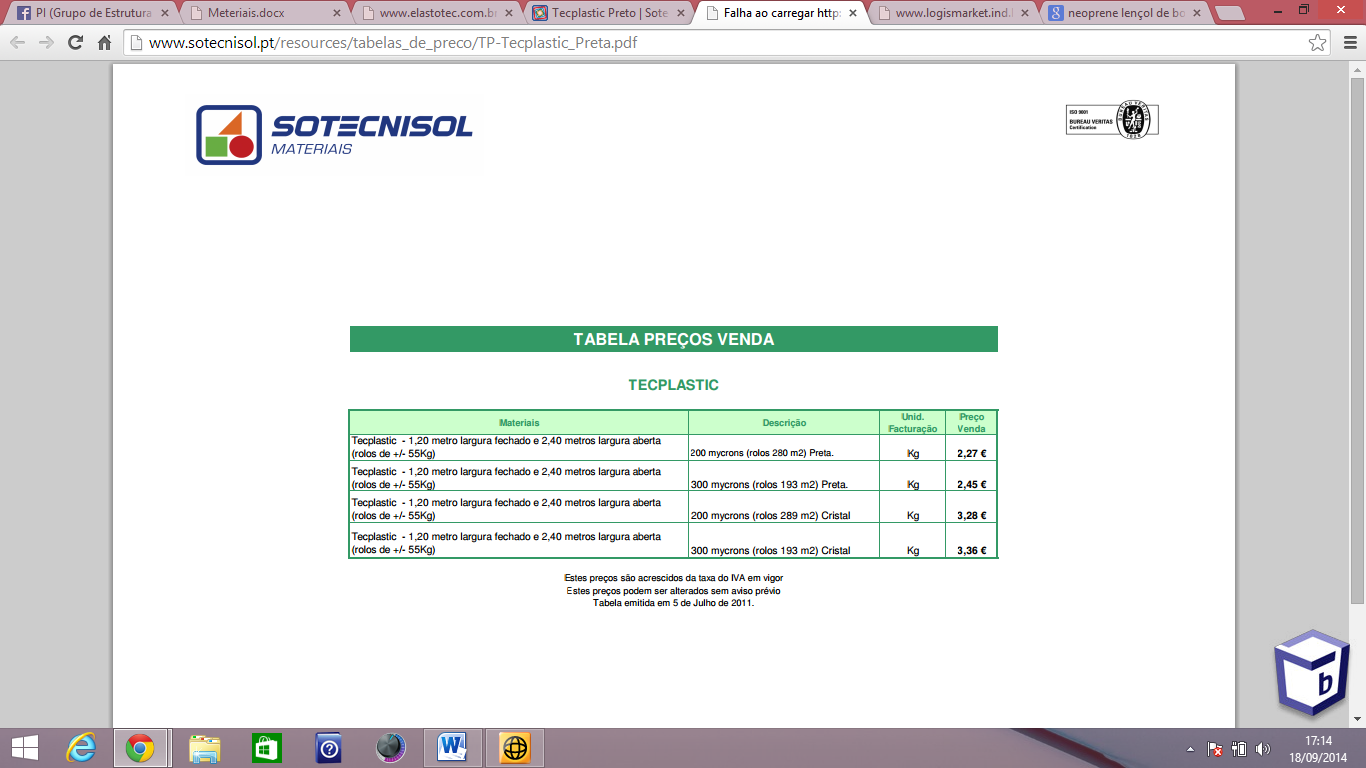
\includegraphics[width=0.8\textwidth]{figuras/preco-polietileno.png}
    \caption{Preços do Polietileno}
    \label{fig:polietileno}
\end{figure} 

Polietileno de Baixa densidade tem sua densidade entre 0,9 e o,95g/cm3, seu ponto de fusão é de 110-115oC, baixa permeabilidade a água, seu módulo de elasticidade está entre 102-204 Mpa, pode ser alongado entre 100-800\% e sua resistência a tração está entre 6,9-16Mpa.

Uma outra alternativa é o nylon(poliamida) ou o decron (poliéster) do tipo rip stop, quando suas tramas e urdume são entrecruzados formando tecidos e a cada 3mm são acrescentados mais três fios para aumentar a resistência ao rasgo, e são impermeabilizados com silicone ou poliuretano que também ajudam a aumentar a resistência contra o desgaste dos raios ultravioleta. Esse tipo de tecido é muito utilizado em balões de balonismo.

Neoprene é formado de policloropreno, o tipo GW tem resistência à água, resistência a rasgo, resistência a flexão dinâmica, suporta temperaturas entre 70-100oC.

\begin{center}
	\begin{tabular}{| l | l | l | l |}
		Material	&	Temperaturas	&	Resistência mecânica	&	Impermeabilidade	\\ \hline
		Borracha natural	&	80-90oC	&	Sim	&	Baixa permeabilidade	\\ \hline
		Polietileno de Baixa Densidade	&	<100oC	&	Sim	&	Baixa Permeabilidade	\\ \hline
		Nylon/Decron	&	-	&	Não muito	&	Permeável	\\ \hline
		Neoprene	&	70-100oC	&	Sim	&	Resistência a agua	\\ \hline
	\end{tabular}
\end{center}

Conclui-se que os materiais podem ser utilizados de maneira eficiente para o revestimento do balão eólica, tendo em vista que atendem as necessidades da mesma. Porém um estudo aprofundado das características e preços ainda deve ser feito para que dentre eles se possa  escolher o mais adequado e viável.

\chapter{Betânia do Piauí}

Para a aplicação do projeto, procurou-se um localidade no Brasil que fosse isolada, com poucos ventos, pouca presença de chuva durante o ano e com problemas de abastecimento energético. Chegou-se, então à cidade de Betânia do Piauí.


\section{Falta de energia elétrica}
   Muitos moradores do município de Betânia do Piauí sofrem com a falta de energia elétrica. O programa Luz para Todos, que visa levar energia elétrica aonde falta, atingiu a região, porém, apenas 373 das 1099 residências de zona rural foram beneficiadas. Parte da dificuldade em atender à todos vem da distância de comunidades em relação à rede existente. 

\section{Clima da região}
O município apresenta temperaturas mínimas de 18°C e máximas de 36°C. Sua altitude é de 480 metros acima do nível do mar. Possui clima semiárido, quente e seco. Os meses mais chuvosos são de dezembro a março. Precipitação anual média em torno de 500mm. 

